\documentclass[tikz,border=8pt]{standalone}
\usepackage[T1]{fontenc}
\usepackage{helvet}
\renewcommand{\familydefault}{\sfdefault}
\usetikzlibrary{arrows.meta, backgrounds}

\definecolor{phasefill}{HTML}{F4F7FB}
\definecolor{phaseborder}{HTML}{9AA7B4}
\definecolor{datafill}{HTML}{FFF4D6}
\definecolor{databorder}{HTML}{D9A441}
\definecolor{llmfill}{HTML}{DFF7F3}
\definecolor{llmborder}{HTML}{1BA99C}
\definecolor{outfill}{HTML}{E7F6E7}
\definecolor{outborder}{HTML}{4FA64F}
\definecolor{darkline}{HTML}{333333}

\tikzset{
  panel/.style={rectangle, rounded corners=10pt, fill=phasefill, draw=phaseborder, line width=1pt},
  box/.style={rectangle, rounded corners=5pt, align=center, draw=darkline, line width=0.8pt, minimum height=0.9cm, font=\small},
  input/.style={box, fill=white, minimum width=2.3cm},
  data/.style={box, fill=datafill, draw=databorder, minimum width=3.2cm},
  llm/.style={box, fill=llmfill, draw=llmborder, minimum width=3.0cm, font=\small\bfseries},
  output/.style={box, fill=outfill, draw=outborder, minimum width=3.0cm},
  context/.style={box, fill=white, minimum width=3.4cm},
  flow/.style={-{Latex[length=2.2mm]}, line width=0.85pt, draw=darkline},
  phase-title/.style={font=\small\bfseries, align=center}
}

\begin{document}
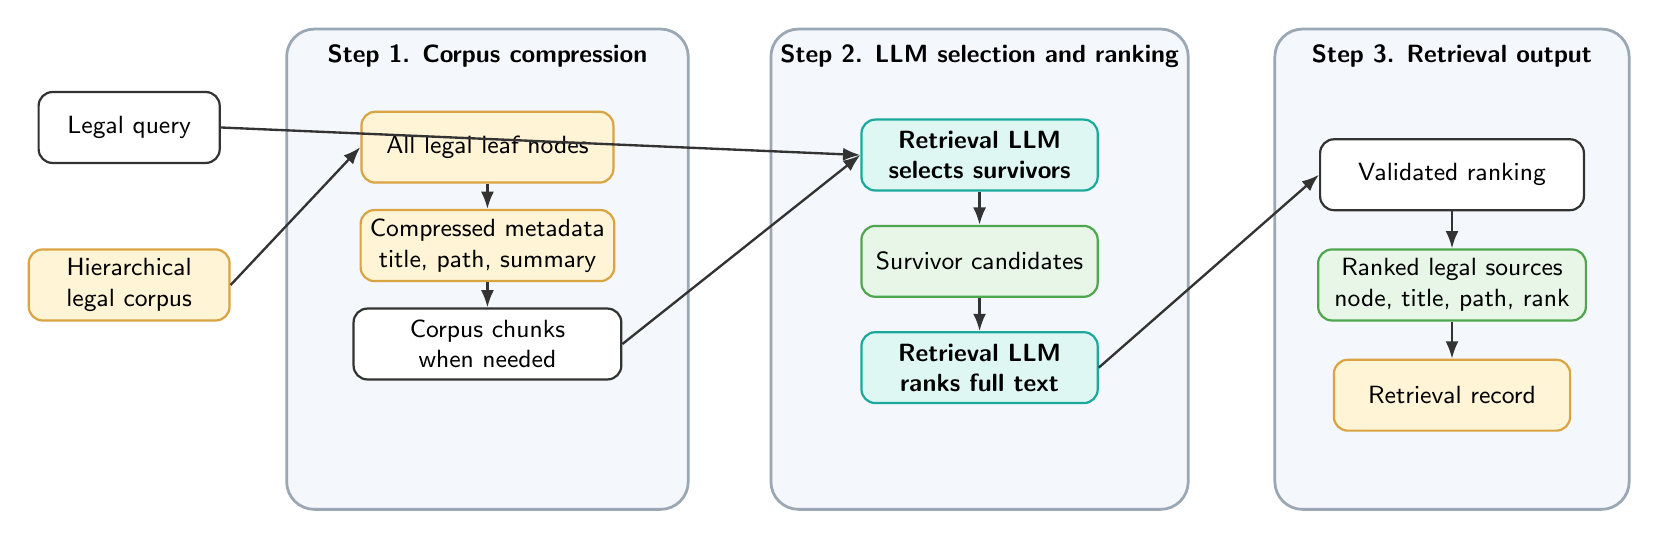
\begin{tikzpicture}

\begin{pgfonlayer}{background}
  \node[panel, minimum width=5.1cm, minimum height=6.1cm] at (4.55, 3.45) {};
  \node[panel, minimum width=5.3cm, minimum height=6.1cm] at (10.8, 3.45) {};
  \node[panel, minimum width=4.5cm, minimum height=6.1cm] at (16.8, 3.45) {};
\end{pgfonlayer}

\node[input] (query) at (0.0, 5.25) {Legal query};
\node[data, minimum width=2.55cm] (corpus) at (0.0, 3.25) {Hierarchical\\legal corpus};

\node[phase-title] at (4.55, 6.15) {Step 1. Corpus compression};
\node[data] (leaves) at (4.55, 5.0) {All legal leaf nodes};
\node[data] (metadata) at (4.55, 3.75) {Compressed metadata\\title, path, summary};
\node[context] (chunks) at (4.55, 2.5) {Corpus chunks\\when needed};

\node[phase-title] at (10.8, 6.15) {Step 2. LLM selection and ranking};
\node[llm] (select) at (10.8, 4.9) {Retrieval LLM\\selects survivors};
\node[output] (survivors) at (10.8, 3.55) {Survivor candidates};
\node[llm] (rank) at (10.8, 2.2) {Retrieval LLM\\ranks full text};

\node[phase-title] at (16.8, 6.15) {Step 3. Retrieval output};
\node[context, minimum width=3.35cm] (validated) at (16.8, 4.65) {Validated ranking};
\node[output, minimum width=3.4cm] (sources) at (16.8, 3.25) {Ranked legal sources\\node, title, path, rank};
\node[data, minimum width=3.0cm] (record) at (16.8, 1.85) {Retrieval record};

\draw[flow] (query.east) -- (select.west);
\draw[flow] (corpus.east) -- (leaves.west);
\draw[flow] (leaves) -- (metadata);
\draw[flow] (metadata) -- (chunks);
\draw[flow] (chunks.east) -- (select.west);
\draw[flow] (select) -- (survivors);
\draw[flow] (survivors) -- (rank);
\draw[flow] (rank.east) -- (validated.west);
\draw[flow] (validated) -- (sources);
\draw[flow] (sources) -- (record);

\end{tikzpicture}
\end{document}
